\documentclass[output=paper]{langsci/langscibook} 
\author{Raphael Berthele\orcid{}\affiliation{University of Fribourg, Institut de Plurilinguisme} and Jan Vanhove\orcid{}\affiliation{University of Fribourg, Institut de Plurilinguisme} and Carina Steiner\orcid{}\affiliation{University of Berne, Center for the Study of Language and Society} and Isabelle Udry\orcid{}\affiliation{University of Fribourg, Institut de Plurilinguisme; Zurich University of Teacher Education} and Hansjakob Schneider\orcid{}\affiliation{Zurich University of Teacher Education}}
\title[Predicting L2 achievement]
      {Predicting L2 achievement: Results from a test battery measuring language aptitude, general learning ability, and affective factors}
\abstract{This chapter addresses the following questions: How, and how accurately, can the children’s performance on a L2 English proficiency test administered around age 12 (T3) be predicted on the basis of test and questionnaire data that were collected one-and-a-half years earlier (T1)? The analyses suggest that a fairly simple equation can predict the score at T3 on new data with an average error of 1.8 points on a 20-point scale. This equation contains seven input variables available at T1. This accuracy corresponds to a R\textsuperscript{2} of 0.58. The seven input variables comprise questionnaire-based affective variables, as well as aptitude measures and German (the pupils’ school language) reading test data. Most of the heavy lifting, however, is done by an English proficiency test administered at T1, which by itself can predict new T3 data with an average error of 2.0 points (R\textsuperscript{2} = 0.41).}
\IfFileExists{../localcommands.tex}{
  \addbibresource{localbibliography.bib}
  % add all extra packages you need to load to this file

\usepackage{tabularx,multicol}
\usepackage{url}
\urlstyle{same}

\usepackage{listings}
\lstset{basicstyle=\ttfamily,tabsize=2,breaklines=true}

%\usepackage{langsci-optional}
\usepackage{langsci-lgr}
\usepackage{langsci-gb4e}
\usepackage{langsci-optional}

\usepackage{enumitem}
\usepackage[group-digits=false, detect-weight=true]{siunitx}

\usepackage{todonotes}

  \newcommand*{\orcid}{}
 
  %% hyphenation points for line breaks
%% Normally, automatic hyphenation in LaTeX is very good
%% If a word is mis-hyphenated, add it to this file
%%
%% add information to TeX file before \begin{document} with:
%% %% hyphenation points for line breaks
%% Normally, automatic hyphenation in LaTeX is very good
%% If a word is mis-hyphenated, add it to this file
%%
%% add information to TeX file before \begin{document} with:
%% %% hyphenation points for line breaks
%% Normally, automatic hyphenation in LaTeX is very good
%% If a word is mis-hyphenated, add it to this file
%%
%% add information to TeX file before \begin{document} with:
%% \include{localhyphenation}
\hyphenation{
affri-ca-te
affri-ca-tes 
Soa-res
scru-ti-ny
me-ta-cog-ni-tion
}

\hyphenation{
affri-ca-te
affri-ca-tes 
Soa-res
scru-ti-ny
me-ta-cog-ni-tion
}

\hyphenation{
affri-ca-te
affri-ca-tes 
Soa-res
scru-ti-ny
me-ta-cog-ni-tion
}
 
  \togglepaper[1]%%chapternumber
}{}

\lehead{Raphael Berthele et al.}
\begin{document}
\maketitle 


\section{Prognostic perspective on aptitude}

Language aptitude testing originated in an interest in prognostic testing. As discussed in Chapter 1, early tests were designed to identify the strong learners within groups of students. This is also one of the research questions of our LAPS project: What is the prognostic value of the aptitude tests for the development of proficiency in the foreign language? The second main question, regarding the underlying structure of individual dispositions to language learning, is discussed in Chapter 3.  Whereas the investigation of dimensionality draws on and contributes to theory building and development regarding the construct of language aptitude, we opted to approach the question of prognostic modelling without a priori theorizing the relative weights of the constructs included in our investigation: We ask how the information gathered at T1 predicts English proficiency 1.5 years later at T3.\footnote{It is, of course, also possible to fit models that predict a student’s performance on the English test at the second data collection using information available at the first or that predict their performance at the third data collection using information available at the first and second. Indeed, in preliminary analyses we also fitted such models. We limit our discussion here to the models we consider the most relevant ones.} The overall aim is to extract a set of predictors that, taken together, would allow teachers to estimate the potential development of their students.

\section{Modelling strategy}

In a first step, our aim is to determine the model that most accurately predicts children’s English proficiency at T3 when all variables assessed in the project are considered (we refer to this as the ‘no costs spared model’). In a second step, we attempt to find a model that is suitable for application in a classroom with comparable predictive value to the no costs spared model. We refer to such a model as the ‘cheap model’. We require that such a model be based on tasks that can be conveniently administered within a 45 minute lesson and evaluated easily by a non-specialist teacher. To this aim, we compared the comprehensive (i.e. no costs spared) model against simpler models, which included background information readily available to the teacher and short tests from our test battery.

The main steps of the process will be summarized in the following. For full details on how we went about building the predictive models, the reader is referred to the technical report \citep{Vanhove2021}. 

\begin{enumerate}
\item Split up the dataset into a training and a test set. The training set was used for trying out different models and for gauging the strength of these different models. Based on the results, the optimal, final model was selected. The test set was used for validating the selected model.
\item Compute scores for constructs such as intrinsic motivation and locus of control. Because of their conceptual and statistical ease of use, we preferred equally-weighted scales wherever they seemed reasonable.
\item Exclude students that are not of interest for the present research question. These are students whose native language is English or who were exempted from English classes. Pupils who did not take the T3 English test were also excluded from the analyses.
\item Reduce the number of predictors. We removed predictor variables with little variance in the training set and we removed one predictor (ELFE total) showing a very strong intercorrelation (0.94) with ELFE word in the training set.
\item Impute missing data. Missing values in the predictor variables that were retained were imputed using the median of the available values of the same variable.
\item Fit models and cross-validate them in the training set. In order to gauge these models’ predictive strength without turning to the test set, cross-validation was applied (section 3.2). This is a technique that essentially mimics the partitioning of the overall dataset into a training and test set (section 3.1). We fitted a whole family of models:

\begin{enumerate}[label=\alph*.]
\item A ‘no-costs spared’ model with all variables assessed.
\item Two simple baseline models so that we could get a sense of how much better the ‘no-costs spared’ model actually performed in cross-validation.
\item Four ‘cheap’ models that could potentially be applied in classroom settings.
\end{enumerate}
\item Select the final models. The final ‘no-costs spared’ and the final ‘cheap’ models were decided on by the research team based on the candidate models’ likely predictive strength (estimated by cross-validation) and, in the case of the ‘cheap’ models, the costs involved in obtaining the predictor information required.
\item Assess the predictive strength of the final model using the test set. The final model was refitted on all of the training data and its predictive strength was then tested on the test set. Importantly, the model’s parameters and settings were not re-estimated or tweaked using the test set.
\end{enumerate}

\section{Data partition and cross-validation}
\subsection{Training and test sets}

Some analyses in this project are exploratory by nature (e.g., the exploratory factor analysis in Chapter 3). Exploratory analyses entail the substantial risk that the models tightly fit the dataset analyzed but do not generalize well beyond it. To offset this risk, we partitioned the dataset analyzed in this chapter into a training set and a test set (see \citealt{KuhnJohnson2013}).

The training set was used to conduct all exploratory analyses and to decide on such matters as data transformations, the calculation of construct scores, missing data imputation, model specification -- in a nutshell, any step in the analysis that requires the analyst to take a decision. Once a suitable predictive model was agreed upon, its predictive power was tested on the test set. Crucially, the chosen predictive model was not re-estimated using the test set data.

To respect the hierarchical nature of the data (children in classes), the test and training sets were not random subsets of the children in the study, but rather (largely) random subsets of the classes in the study (see \citealt{RobertsEtAl2017}). In this way, we could account for the clustering of the pupils in classes when estimating the prediction error in our models. Specifically, from the 17 grade 4 classes at T1, 5 were selected to comprise the test set: the smallest class (Class 4, with 5 grade 4 pupils at T1)\footnote{The sometimes small number of pupils per class is a consequence of some of the classes being mixed grade.} as well as four randomly picked classes. Similarly, from the 19 grade 5 classes at T1, 6 were selected to comprise the test set: the smallest class (also Class 4, with only 1 grade 5 pupil at T1) as well as five randomly picked classes. The remaining 12 grade 4 and 13 grade 5 classes comprised the training set.


\begin{table}
\caption{Training and test sets. \emph{Note:} The number of classes sums to 36 rather than 32 because four classes had pupils from both 4th and 5th grade at T1. Only pupils for whom T3 English sores were available were included in the predictive models; for the final models, we only included participants who also had T1 English scores.\label{tab:04:1}}
\begin{tabular}{ll *{3}{c}}
\lsptoprule
{Set} & {Cohort} & {Classes} & \multicolumn{2}{c}{English data at}\\\cmidrule(lr){4-5}
      &          &           & {T3 only} & {both T1 and T3}\\\midrule
{Training} & {4th grade at T1} & {12} & {169} & {154}\\
           & {5th grade at T1} & {13} & {187} & {177}\\
{Test}     & {4th grade at T1} & {5} & {70} & {65}\\
           & {5th grade at T1} & {6} & {85} & {80}\\
\lspbottomrule
\end{tabular}
\end{table}


\subsection{Cross-validation}

When trying out different models on the training data, we used cross-validation to estimate how well the models would work for new data.\footnote{This section is adapted from \citet{VanhoveEtAl2019}.} This was done to ensure that overzealous data exploration and model fine-tuning would not result in a model that fits the training data well but stands little chance of predicting the test data (see \citealt{KuhnJohnson2013}; \citealt{YarkoniWestfall2017}). In cross-validation, the training data is split up into a number ($k$) of folds, and models are fitted on $k-1$ folds and then used to predict the outcome in the remaining fold. This process is repeated $k$ times, each time leaving out a different fold. The result is $k$ estimates of the models’ predictive accuracy on data not used for fitting the model that can then be averaged. The folds were not constructed randomly, since we need to account for the dependency structure in the data (pupils in classes). Therefore, we opted for block cross-validation, using each class as a separate fold.

Figure 1 illustrates the principles behind the partitioning of the data and block cross-validation.


\begin{figure}
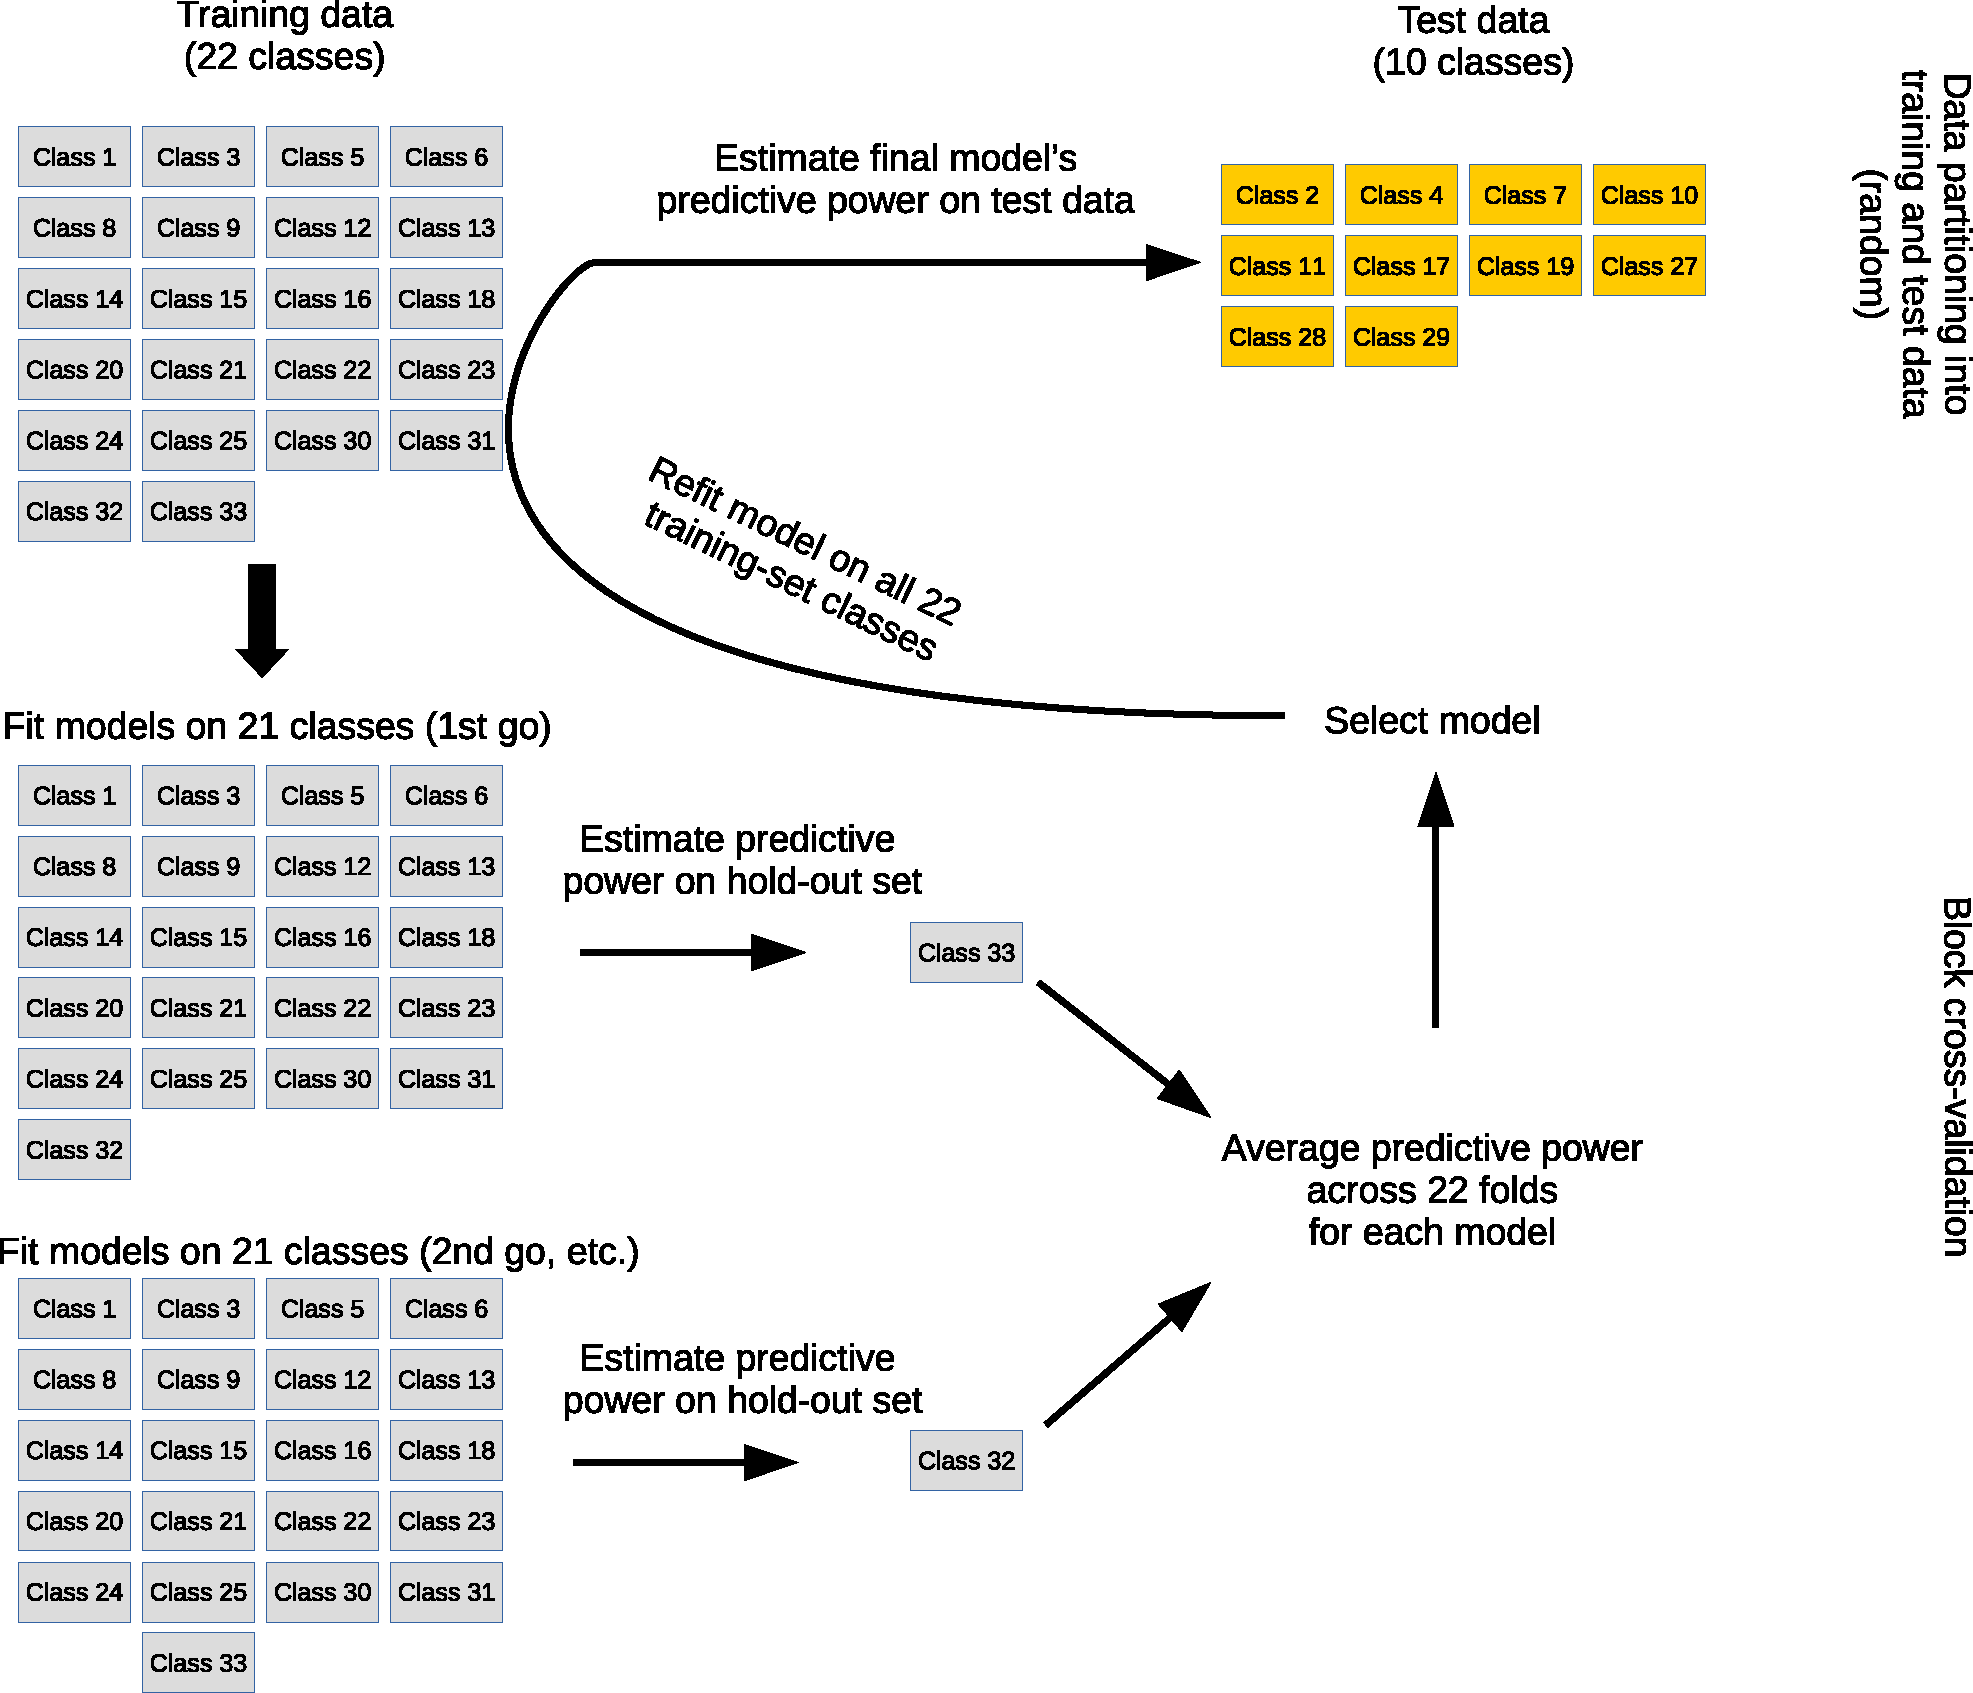
\includegraphics[width=\textwidth]{figures/figure4.1.cross-validation.pdf}
\caption{Illustration of how the data were partitioned into a training ($N=356$) and a test set ($N=155$) and of how block cross-validation works. Only two iterations of block cross-validation are shown; in reality, 22 took place for each model, each time leaving out a different class. Figure based on Figure~3 in \citet{VanhoveEtAl2019}.}
\label{fig:04:1}
\end{figure}

\subsection{Metrics of model performance}

The root mean squared error (RMSE) was used to adjudicate between different models. The RMSE can be interpreted as being roughly – but not quite – the average difference between a model’s predictions and the observed values. (In the same way that a standard deviation can be interpreted as being roughly – but not quite – the average difference between the observations and their mean.) The interpretation of the mean absolute error (MAE) is simpler: It is the average (mean) difference between a model’s prediction and the observed values. We report both metrics in this chapter.

Many readers will be more familiar with the R\textsuperscript{2} metric of (so-called) ‘explained’ variance. Several problems beset R\textsuperscript{2}, but perhaps most important of all is that R\textsuperscript{2}, as it is traditionally computed, does \textit{not} estimate how well the model itself would capture the variance in a new sample. Instead, it estimates (at best) how well a \textit{newly estimated} model would capture the variance in a new sample.\footnote{There exist different ways of computing R\textsuperscript{2} (Kvålseth, 1985). For ordinary regression models, these all yield the same result. However, when the model is used to predict observations that were not used when fitting the model, they do not. One popular method for computing R\textsuperscript{2} is to square the correlation between the predicted and observed values. This is problematic since the correlation between predicted and observed values can be excellent even if the former corresponds poorly to the latter (e.g., the values 1, 2, 3 correlate perfectly with the values 2000, 4000, 6000 but correspond poorly to them). We therefore computed R\textsuperscript{2} as the proportional decrease in the residual sum of squares relative to a baseline model without any predictors. Such a model predicts each new observation to be equal to the mean of the training data. (Footnote adapted from \citealt{VanhoveEtAl2019})}

\section{Selection of the ‘no costs spared’ model}

As shown in \tabref{tab:04:1}, the training set for T3 comprised 169 4\textsuperscript{th} graders and 187 5\textsuperscript{th} graders. The test set comprised 70 4\textsuperscript{th} graders and 85 5\textsuperscript{th} graders.

To fit the ‘no-costs spared’ model, all available T1 information, from all possible sources, was allowed to enter into this model, without regard to how difficult or costly it was to collect this information. 

To arrive at the final model in this category, a host of models were fitted on the training data. These included multiple linear regression, robust regression, ridge regression, elastic net, multivariate adaptive regression splines, generalized additive models, partial least squares regression, k-nearest neighbors, regression trees, random forests, support vector machines, stochastic gradient boosting, and Cubist.\footnote{For details on the architecture of these models, see www.osf.io} A multiple linear model with seven predictors and no interactions (\tabref{tab:04:2}) performed roughly on par with the more complex approaches in cross-validation. When fitting the final model, we only took into account participants who had T1 English test scores. The model’s estimated coefficients are shown in \tabref{tab:04:2}. 

We want to draw the attention of any reader who wishes to use this model for understanding (as opposed to predicting) foreign-language learning to what \citet{Breiman2001} calls the ‘Rashomon effect’: While the presented model worked best in cross-validation, a number of models with different predictors fared only slightly worse. Consequently, one would be jumping to conclusions if one said that the seven predictors listed in \tabref{tab:04:2} are important in foreign-language learning and the others are not. The performance of the more complex models in cross-validation can be consulted in the online materials (\url{https://osf.io/ha7s2/}).


\begin{table}
\caption{Multiple linear regression model for predicting T3 English scores. \emph{Note:} Missing predictor data were imputed using median imputation using the full training set data. Median = the predictor’s median in the training set (used in imputation). Estimate = the estimated regression coefficient for the predictor. SE = the naïve standard deviation for the estimated regression coefficient; naïve meaning that its computation did not take into account the fact that this model was selected for its performance in cross-validation.\label{tab:04:2}}
\begin{tabular}{l SSS}
\lsptoprule
 {Term} & {Median} & {Estimate} & {SE}\\\midrule
Intercept &  & 0.045 & 1.4\\
English T1 & 49 & 0.093 & 0.010\\
Grade at T1 & 5 & -0.55 & 0.31\\
Intrinsic motivation & 3 & 0.48 & 0.22\\
Self-concept English & 3 & 0.89 & 0.22\\
German (ELFE sentences/minute) & 7.33 & 0.49 & 0.08\\
Grammatical sensitivity (gra) & 15 & 0.047 & 0.023\\
Inductive ability (ind) & 5 & 0.16 & 0.05\\
\lspbottomrule
\end{tabular}
\end{table}


Second, we fitted two simple baseline models so that we could get a sense of how much better the ‘no-costs spared’ model actually performed in cross-validation. The first baseline model was a ‘no predictor’ model, which predicted each unseen data point to be equal to the mean of the seen data points. The second was an ‘English-only’ model, which only contained the participants’ T1 English test score as the predictor of their T3 English test score. This was done because the English score at T1 unsurprisingly explains the largest share of variance of English at T3 since it taps into the same construct.

In cross-validation, the no costs spared model (\tabref{tab:04:2}) with seven predictors fitted the data better than the baseline models, the residual sum of squares is reduced by about 58\% relative to an intercept-only model (i.e., $\smash{\text{R}^2_{\text{RSS}}}$ = 0.58, 95\% CI: [0.49, 0.66]). 

The no costs spared model’s root mean square error (RMSE) in cross-validation was 2.24 (95\% CI: [2.02, 2.47]), and its mean absolute error (MAE) in cross-validation was 1.77 (95\% CI: [1.60, 1.95]). For reference, an intercept-only model yielded a RMSE of 3.69 and a MAE of 2.93. A linear model with a single predictor, viz., the participants’ English score at T1, was also fitted and cross-validated. This model yielded $\smash{\text{R}^2_{\text{RSS}}}$ = 0.42, RMSE = 2.61 and MAE = 2.03. These results from the cross-validation analysis, also shown in \figref{fig:04:2}, suggest that there is a considerable gain in predictive performance when English at T1 is used, and some further gain when, in addition to English at T1, the other six predictors from \tabref{tab:04:2} are included.

When applied to the test set, the linear model with seven predictors reduced the residual sum of squares by about 62\% relative to the intercept-only model (i.e., R\textsuperscript{2} = 0.62, 95\% CI: [0.52, 0.70]). Its root mean square error (RMSE) was 2.32 (95\% CI: [2.02, 2.60]) and its mean absolute error (MAE) 1.85 (95\% CI: [1.63, 2.08]).

These results are summarized in \figref{fig:04:2}. 



\begin{figure}
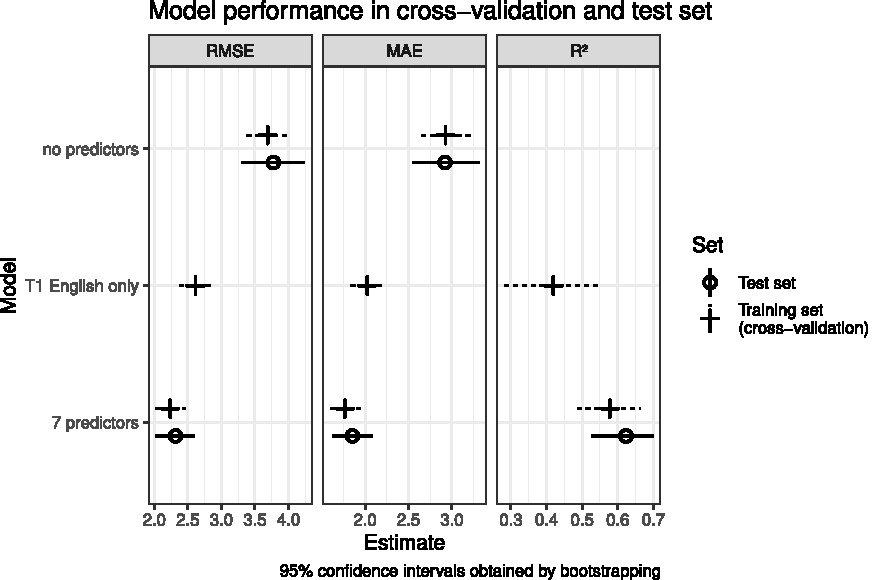
\includegraphics[width=\textwidth]{figures/Figure4.2.model_comparison-bw.pdf}
\caption{Performance of the chosen model relative to two baseline models. Note. The R\textsuperscript{2} value for the intercept-only model is not shown as it is 0 by definition. The 95\% confidence intervals were obtained by bootstrapping the 22 cross-validation estimates or by bootstrapping the observed and predicted test set values and recomputing the estimates (percentile approach). The English-only model wasn’t applied to the test set.\label{fig:04:2}}
\end{figure}

\subsection{Selection of the ‘cheap’ models}

Next, we fitted four models that include sets of variables that are less costly to acquire or even completely ‘free’ in the sense that the required information on the pupils is usually a given in the school context. We refer to these models as ‘cheap’ models. They could be used in a classroom setting without having to collect data during four full lessons, the required time for the full LAPS test battery. The rationale here is to explore the possibility of predicting foreign language achievement based on information that is not complicated to get. 

Free variables encode information that is available to teachers anyway as opposed to, say, a computer-based test of working memory. Information included as “free variables” were whether students had additional support in class, grade, and whether their L1 was German. This only involves information that wouldn’t lead to discrimination based on sex (no gender variable) or possibly socio-economic background (no SES variable from the parent questionnaire). 

Relatively ‘cheap variables’ are measures that are easy to take (paper and pencil instruments in the case of the aptitude tests, or questionnaire items on motivation). In this selection process, we also took into consideration a small set of measures that are somewhat less straightforward to acquire (since they need to be purchased and/or adapted), such as language tests and aptitude tasks, but that are highly relevant to the central constructs of our investigation. Included here were thus T1 English score (OYLPT), T1 German score (ELFE), T1 motivation questionnaire-based construct scores, and the inductive ability score (PLAB form 4).

Four cheap models were fitted. The first one includes English at T1 and all the free variables mentioned above. The second includes reading skills in the school language (German) and all free variables. The third includes the motivational items regarding English and the free variables, and the last one motivational items and the adaptation of the PLAB subtest of inductive learning. The performance of these four models on the test set are given in \tabref{tab:04:3}. 


\begin{table}
\caption{The four cheap models and their performance on the training and (for two of them) test sets. Tr: Training set; Te: Test set. \emph{Note:} The training set estimates were obtained through cross-validation.\label{tab:04:3}}
\begin{tabular}{l cc cc cc}
\lsptoprule
 Model no. \& included variables & \multicolumn{2}{c}{RMSE} & \multicolumn{2}{c}{MAE} & \multicolumn{2}{c}{R\textsuperscript{2}}\\\cmidrule(lr){2-3}\cmidrule(lr){4-5}\cmidrule(lr){6-7}
                             &  Tr & Te &  Tr & Te &  Tr & Te\\\midrule
1 English T1 + free variables & 2.48 & 2.52 & 1.99 & 1.96 & 0.47 & 0.55\\
2 L1 German (ELFE) + free variables & 2.69 &  & 2.19 &  & 0.39 & \\
3 Motivation + free variables & 2.83 &  & 2.27 &  & 0.34 & \\
4 Motivation + ind + free variables & 2.69 & 2.82 & 2.16 & 2.24 & 0.40 & 0.46\\
\lspbottomrule
\end{tabular}
\textup{}
\end{table}


Our research group then discussed which ones of these cheap models should be validated on the test set. For the reasons spelled out above, most importantly to avoid over-fitting, we wanted to select a maximum of two models. Given the known strong association of the English at T1 test with our outcome variable at T3, the first cheap model was to be retained. The second model selected was the next best model according to the MAE and RMSE performance on the training set. This model includes motivational items and the inductive ability test based on a form of the PLAB.\footnote{With the kind permission of Charles Stansfield, LLTF, we adapted this form of the PLAB without having to pay any fees. If, however, a German version of PLAB should be developed in the future, this would most likely not be free to use.} The first and fourth model were then applied to the test set. When applied to the test set, the cheap model 1 (English at T1 and all of the free variables) did better than the cheap model 4 (motivation, inductive ability and free variables). As a reminder, the free variables contain information that is often known anyway to teachers (and if not readily available), e.g. whether students had additional support in class, the pupils’ current grade, and whether one of their L1 was German. This cheap model 1 has an R\textsuperscript{2} of 0.47 on the training set and of 0.55 on the test set. 

\section{Discussion}

The general goal of the analysis presented in this chapter was to assess the possibility to prognosticate foreign language development in primary school children. As discussed in Chapter 1, prognostication was what inspired the first practitioners and scholars to develop modern language aptitude tests: Predicting the success in learning a new language would help select the ‘apt’ learners and prevent spending time and money on not so apt individuals. Most of this research and development focused on (young) adults and adolescents.

Our primary goal was not to provide an instrument for selection –  foreign language education in the context investigated here is compulsory anyway. However, prognostication can serve other purposes as well (see Chapter 11 for a discussion).

Our attempt to investigate prognostication took several alternative paths. The first path, the ‘no costs spared’ approach, took all information available at T1 into consideration. The multi-step modelling procedure explained in this chapter yields a model that we expect to predict the English score (on a scale from 0 to 20) of new data with a mean absolute error of about 1.8 points. Whether this is a good or a bad model performance depends on the criteria one wishes to apply. It certainly shows that the development in the foreign language is not simply random but is constrained by some of the constructs known and used in research on individual differences in language learning. Among the seven predictors in the model that showed the best performance on our test set, we find both emotional/motivational variables (intrinsic motivation, self-concept) and language-related variables (grammatical sensitivity [based on MLAT-E part 2] and inductive ability [based on PLAB, form 4], but also German reading proficiency). 

The fact that the English skills tested one and a half years before T3 is the best predictor for the same skill is not surprising. But it also shows that, within the time interval covered by this study, relative differences in English skills are retained (see Chapter 10 for an analysis of the intra-individual stability across time of other constructs). 

As discussed above, other models with different sets of predictors show almost the same performance (Rashomon effect). The list of variables of our best model therefore is not to be read as a final list of predictors of success in foreign language learning, implying that the variables not retained are not important. What our analyses merely show is that these measures are robustly associated with foreign language development, even when we apply cautious modelling that aims at avoiding over-fitting the data. In support of the relevance regarding the variables just mentioned, we can also refer to the cross-sectional analysis discussed in Chapter 3 where we show that these variables are part of the two constructs that are positively associated with English skills at T1 (we labelled these factors \textit{Cognition/Aptitude} and \textit{L2} \textit{Academic Emotion}).

Among this first set of models that yield the optimal ‘no cost spared model’, we found that a simple model with T1 English as its sole predictor performs roughly on par with the other, more complex models (state estimate of about 2 on a scale 0-20). 

After this first analysis, we took a less maximalist but more pragmatic perspective on prognostication. This involved fitting four ‘cheap’ models to the data sets. In certain pedagogical contexts, it can be useful to assess individual differences in foreign language learning with relatively simple tests. Thus, we compared different sets of tests with respect to their prognostic values. All of them can be administered in a classroom setting and do not take up more than 45 minutes. These models include only variables that are already available to the teacher or that do not require complicated testing procedures. From these cheap models, the one with the T1 English test score plus the free variables and the one with Motivation plus the inductive ability test from the PLAB plus the free variables were selected and applied to the test set. Based on a comparison of the performance of these models, it appears reasonable to use the Oxford Young Learners Placement Test plus the set of information we termed the ‘free variables’ for prognostic use. This test of English skills is not freely available (it currently costs around £5 per pupil) and it would be a matter of choice on the part of the teachers or schools whether they would wish to consider such a test. 

The analysis in this chapter aims to identify the best combination of measures taken at T1 to predict English skills at T3. The models discussed here, and their variable prognostic performance, are not designed with the goal to disentangle the different dimensions of predispositions for language learning. This was the main goal of the analyses in Chapter 3. Despite the different questions asked in Chapters 3 and 4, it seems reassuring that when looking at the list of variables in our no costs spared model (\tabref{tab:04:2}), we find tests that are all loading onto one of the two factors that are positively associated with English skills at T1, that is measures we subsumed under the two labels cognition/aptitude and L2 academic emotion in Chapter 3. As in that preceding chapter’s analyses, extrinsic motivational constructs are not first in line when their association with English skills is investigated. 

{\sloppy\printbibliography[heading=subbibliography,notkeyword=this]}
\end{document}
